% ======================================================================
\section{Experiments}\label{sec:exp}
% ======================================================================
\subsection{Setup}\label{sec:setup}
\paragraph*{Compared methods}
\emph{Zero-shot terrestrial models} use their official weights: CosPlace-R50~\cite{berton2022cosplace}
($512$-D), EigenPlaces-R50~\cite{berton2023eigenplaces} ($2048$-D) and DINOv2-SALAD~\cite{izquierdo2024optimal}
($8448$-D, trained on GSV-Cities~\cite{alibey2022gsv}). \emph{Lunar-trained heads} all share the
frozen SALAD-fine-tuned DINOv2 ViT-B/14 backbone, the training data, the loss and the schedule, and
differ only in the aggregation: GeM~\cite{radenovic2019gem} ($1280$-D), NetVLAD~\cite{arandjelovic2016netvlad}
($k$-means-initialised, $64\times128$ + scene token, $8448$-D), SALAD (balanced OT, $\lambda=1$) and
Galatea (semi-relaxed UOT with learned $\lambda$). The last three have identical descriptor size
and almost identical parameter counts. For stage~2 we compare four local scorers on the same
SuperPoint keypoints (top $384$ by score) and top-$K=10$ candidates: mutual nearest neighbours
with cosine $>0.7$ (MNN), training-free entropic OT with dust-bins (UOT, appearance only), the learned LightGlue
matcher~\cite{lindenberger2023lightglue}, and our partial FGW. Each is used with and without
MAGSAC++ verification.

\paragraph*{Implementation}
Images are resized to $210\times280$ for the ViT ($n=300$ tokens). Heads are trained with AdamW
(learning rate $4\cdot10^{-4}$, one-cycle schedule, weight decay $10^{-4}$) for $500$ steps of $24$
places $\times$ $4$ views, using the multi-similarity loss ($\alpha=1$, $\beta=50$, miner margin $0.1$).
Sinkhorn uses $L=3$ iterations, $m=64$ clusters and $\ell=128$. The four main heads and the $\lambda=0$ ablation
are run with three seeds (mean $\pm$ standard deviation); the other ablations use one seed. For stage~2, the structural weight $\alpha\in\{0,0.3,0.6\}$ (chosen: $0.3$) and the fusion
parameters $\beta,\kappa$ are selected on the validation scene only. $\varepsilon_\ell=0.05$ and the
dust-bin cost threshold $0.25$ (cosine $0.75$) are fixed a priori, and MAGSAC++ uses a $1.5$\,px threshold. All experiments run on a $2$-core CPU without a GPU. Code, the renderer, the rendered
benchmark and the trained heads are available at \url{https://github.com/RaunakDune/galatea-lunar-vpr}.


\begin{figure*}[t]
\centering
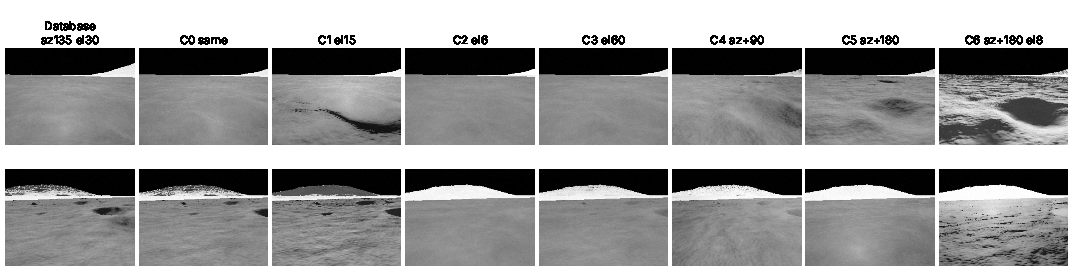
\includegraphics[width=\textwidth]{figures/conditions.pdf}
\caption{LunarSim-VPR: two test places (rows). Left: database image (Sun azimuth $135^\circ$,
elevation $30^\circ$). Right: queries at a jittered pose under the seven Sun conditions of
\cref{tab:conds}. Rendered with lunar-Lambert photometry, opposition surge and cast shadows from
local and regional relief. In the top row at C2, the camera lies in the shadow of a distant massif
and is lit only by the weak ambient term.}
\label{fig:conds}
\end{figure*}
\begin{figure}[t]
\centering
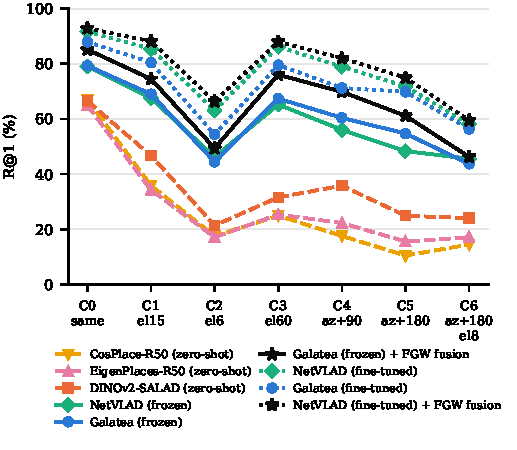
\includegraphics[width=\columnwidth]{figures/percond.pdf}
\caption{R@1 per illumination condition on the test set. Zero-shot terrestrial models (dashed)
collapse once the Sun moves. Lunar-trained OT aggregation (Galatea) and global--local fusion
(Galatea + FGW) recover much of the loss, most of all under shadow reversal and grazing light.}
\label{fig:percond}
\end{figure}

\begin{table*}[t]
\centering
\caption{Recall (\%) on the LunarSim-VPR test set (3 unseen scenes, 3150 queries). Lunar-trained heads share the frozen DINOv2 backbone and training protocol; mean$\pm$std over 3 seeds. Per-condition columns give R@1 (conditions in \cref{tab:conds}).}
\label{tab:main}
\footnotesize
\setlength{\tabcolsep}{4pt}
\begin{tabular}{@{}llr ccc ccccccc@{}}
\toprule
& Method & Dim. & R@1 & R@5 & R@10 & C0 & C1 & C2 & C3 & C4 & C5 & C6 \\
\midrule
\multirow{3}{*}{\rotatebox{90}{\scriptsize zero-shot}} & CosPlace-R50~\cite{berton2022cosplace} & 512 & 26.8 & 50.3 & 60.8 & 66.9 & 35.8 & 17.6 & 24.9 & 17.6 & 10.4 & 14.4 \\
 & EigenPlaces-R50~\cite{berton2023eigenplaces} & 2048 & 28.1 & 53.0 & 64.1 & 64.9 & 34.2 & 17.1 & 25.3 & 22.2 & 15.6 & 17.1 \\
 & DINOv2-SALAD~\cite{izquierdo2024optimal} & 8448 & 35.8 & 65.4 & 77.7 & 66.4 & 46.7 & 21.3 & 31.6 & 35.8 & 24.9 & 24.0 \\
\midrule
\multirow{4}{*}{\rotatebox{90}{\scriptsize lunar-trained}} & GeM & 1280 & 31.5{\scriptsize$\pm$0.4} & 64.7{\scriptsize$\pm$0.3} & 79.4{\scriptsize$\pm$0.2} & 55.0 & 34.8 & 19.8 & 35.3 & 30.1 & 25.1 & 20.3 \\
 & NetVLAD & 8448 & 58.2{\scriptsize$\pm$0.7} & 86.6{\scriptsize$\pm$0.4} & 94.6{\scriptsize$\pm$0.2} & 79.0 & 67.5 & 46.1 & 65.2 & 56.0 & 48.3 & 45.6 \\
 & SALAD ($\lambda{=}1$) & 8448 & 59.4{\scriptsize$\pm$0.7} & \textbf{87.3{\scriptsize$\pm$0.7}} & \textbf{94.8{\scriptsize$\pm$0.2}} & 77.6 & 68.4 & \textbf{46.4} & 65.4 & 58.6 & 52.7 & \textbf{46.7} \\
 & Galatea, learned $\lambda$ & 8448 & \textbf{59.8{\scriptsize$\pm$0.8}} & \textbf{87.3{\scriptsize$\pm$0.5}} & 94.6{\scriptsize$\pm$0.2} & \textbf{79.3} & \textbf{69.0} & 44.4 & \textbf{67.3} & \textbf{60.4} & \textbf{54.7} & 43.7 \\
\bottomrule
\end{tabular}
\end{table*}

\subsection{Terrestrial models under lunar illumination change}\label{sec:zeroshot}
\Cref{tab:main} (top) shows that all three terrestrial models perform reasonably when only the
viewpoint changes: at C0, R@1 is $\zsEigCzero$--$\zsCosCzero\%$. They degrade sharply as soon as the
Sun moves. DINOv2-SALAD, the strongest of them, falls from $\zsSaladCzero\%$ at C0 to
$\zsSaladCtwo\%$ under grazing illumination (C2) and to $\zsSaladCfive\%$ when the shadows flip (C5).
The CNN-based CosPlace and EigenPlaces fare worse, with C5 values of $\zsCosCfive\%$ and $\zsEigCfive\%$.
Even a foundation-model backbone pre-trained on 142M images therefore does not provide
illumination-invariant place descriptors on regolith. Local re-ranking does not close the gap
either. Fusing MNN+MAGSAC++ matches into the top-10 zero-shot SALAD candidates (selected on
validation as in \cref{sec:rerank}) raises R@1 to $\zsRRRone\%$. That is still below the lunar-trained
stage~1 \emph{without} re-ranking, and only $\zsRRHard\%$ on the hardest conditions, because the
correct place is often not among the candidates at all.

\subsection{Lunar-adapted OT aggregation}\label{sec:stage1}
Training only the aggregation head on illumination-diverse LunarSim scenes (backbone frozen) lifts
R@1 from $\zsSaladRone\%$ to $\galRone\%$ (Galatea, mean of three seeds). On the paired test queries
this is a gain of $\gainZsMean$ points (95\% CI $[\gainZsLo,\gainZsHi]$). The largest gains are under
illumination change. Mean R@1 over the three hardest conditions (C2, C5, C6) rises from $\zsSaladHard\%$
to $\galHard\%$. The three cluster-based heads (NetVLAD, SALAD and Galatea) clearly beat every zero-shot model.
GeM pooling of the same frozen tokens does not ($\gemRone\%$). Without fine-tuning the backbone,
global pooling cannot separate place-specific tokens from illumination-dependent ones, while
cluster-based aggregation can~\cite{izquierdo2024optimal}.

Galatea and SALAD are statistically indistinguishable: the paired difference in R@1 is
$\galVsSalMean$ points (95\% CI $[\galVsSalLo,\galVsSalHi]$), as \cref{prop:colinv} predicts. The two heads differ sharply in how they spend mass. The balanced head sends
$\salDust\%$ of all token mass to the dust-bin, and its total dust-bin mass correlates with the sky
fraction of the image ($\rho=\salSkyCorr$). The learned unbalanced head ($\bar\lambda=\galLam$)
discards only $\galDust\%$ and concentrates the remaining mass on a few clusters (coefficient of
variation of cluster mass $\galCV$ vs.\ $\salCV$). Their retrieval performance is nevertheless the
same. On this data, therefore, the assignment's marginal constraints are not the bottleneck; the
training distribution is. We return to this in \cref{sec:ablation}.

\begin{table}[t]
\centering
\caption{Stage-2 re-ranking of the top-10 Galatea candidates (test, \%). \emph{Local}: sort by the local score only. \emph{Fused}: \cref{eq:fusion} with $(\beta,\kappa)$ chosen on the validation scene.}
\label{tab:rerank}
\footnotesize
\setlength{\tabcolsep}{3pt}
\begin{tabular}{@{}lcccc@{}}
\toprule
& \multicolumn{2}{c}{Local} & \multicolumn{2}{c}{Fused} \\
\cmidrule(lr){2-3}\cmidrule(lr){4-5}
Local scorer & R@1 & R@5 & R@1 & R@5 \\
\midrule
none (global ranking) & \multicolumn{2}{c}{--} & 60.8 & 88.0 \\
MNN & 59.2 & 88.2 & 66.0 & 89.5 \\
MNN + MAGSAC++ & 62.4 & 89.2 & \textbf{67.2} & 90.0 \\
OT, appearance only & 57.0 & 89.5 & 65.8 & 90.4 \\
OT, appearance only + MAGSAC++ & 61.0 & 88.3 & 63.0 & 88.6 \\
LightGlue~\cite{lindenberger2023lightglue} (learned) & 57.5 & 87.4 & 65.3 & 89.6 \\
LightGlue~\cite{lindenberger2023lightglue} (learned) + MAGSAC++ & 60.0 & 89.0 & 65.7 & 89.8 \\
Partial FGW (ours) & 59.8 & 90.1 & 66.0 & 90.1 \\
Partial FGW (ours) + MAGSAC++ & 63.0 & 88.6 & 63.8 & 88.7 \\
\bottomrule
\end{tabular}
\end{table}

\subsection{Global--local fusion with OT re-ranking}\label{sec:rerank}
\Cref{tab:rerank} re-ranks the top-10 candidates of Galatea (seed 0, R@1 $\rrGlobRone\%$).
Two findings stand out. First, ranking by the local score alone barely helps and can hurt: no scorer
improves R@1 by more than about two points, and several lose ground. The reason is that SuperPoint
responses on regolith are dominated by shadow edges, which move with the Sun. Second, fusing local
and global evidence with \cref{eq:fusion} helps every scorer. With partial FGW, R@1 rises to
$\rrFgwRone\%$, a gain of $\rrGainMean$ points (95\% CI $[\rrGainLo,\rrGainHi]$), and on the hardest
conditions from $\galSzeroHard\%$ to $\rrFgwHard\%$, the best of all scorers on that subset.
Differences between scorers in the fused setting are small and within the confidence intervals:
FGW vs.\ LightGlue $\fgwVsLgMean$ $[\fgwVsLgLo,\fgwVsLgHi]$, and FGW vs.\ appearance-only OT
$\fgwVsUotMean$ $[\fgwVsUotLo,\fgwVsUotHi]$. The training-free structural matcher thus performs as
well as a learned terrestrial matcher. MAGSAC++ helps MNN and LightGlue but not the OT matchers, whose dust-bins already reject outliers.
The effect is robust across stage-1 seeds. Repeating the protocol on all three Galatea seeds
(re-tuning $\beta,\kappa$ on validation each time), fusion gains $\msFgwGain\pm\msFgwGainsd$ points R@1
with FGW, $\msMnnRGain\pm\msMnnRGainsd$ with MNN+MAGSAC++ and $\msMnnGain\pm\msMnnGainsd$ with plain MNN.
The practical lesson is that, on the Moon, \emph{how local and global evidence are combined matters
more than which local matcher is used}.

\begin{table}[t]
\centering
\caption{Ablations of the stage-1 aggregator (test R@1/R@5, \%; hard = mean R@1 over C2, C5, C6). Top: assignment relaxation $\lambda$ (mean$\pm$std over the seeds available; single-seed rows marked $^\dagger$). Bottom: Galatea variants vs.\ the seed-0 reference.}
\label{tab:ablation}
\footnotesize
\setlength{\tabcolsep}{3.5pt}
\begin{tabular}{@{}lccc@{}}
\toprule
Variant & R@1 & R@5 & hard \\
\midrule
$\lambda=0$ (NetVLAD assignment + dust-bin) & 59.9{\scriptsize$\pm$0.8} & 87.6{\scriptsize$\pm$0.6} & 48.4 \\
$\lambda=0.25$ (fixed)$^\dagger$ & 60.7 & 88.2 & 48.1 \\
$\lambda$ learned (Galatea, init.\ 0.5) ($\bar\lambda{=}0.50$) & 59.8{\scriptsize$\pm$0.8} & 87.3{\scriptsize$\pm$0.5} & 47.6 \\
$\lambda$ learned, $25\times$ lr on $\lambda,z$ ($\bar\lambda{=}0.56$)$^\dagger$ & 60.3 & 87.7 & 47.3 \\
$\lambda=0.75$ (fixed)$^\dagger$ & 59.2 & 87.9 & 48.2 \\
$\lambda=1$ (SALAD, balanced) & 59.4{\scriptsize$\pm$0.7} & 87.3{\scriptsize$\pm$0.7} & 48.6 \\
\midrule
Galatea (seed 0, reference) & 60.8 & 88.0 & 47.8 \\
\quad no dust-bin & 62.1 & 88.0 & 49.3 \\
\quad $L=1$ Sinkhorn iteration & 59.9 & 87.8 & 46.6 \\
\quad $L=10$ iterations & 60.7 & 88.0 & 47.7 \\
\quad $m=16$ clusters & 57.7 & 86.2 & 45.9 \\
\quad $m=32$ clusters & 61.1 & 88.2 & 47.9 \\
\quad single-illumination training & 47.3 & 72.2 & 27.6 \\
\bottomrule
\end{tabular}
\end{table}

\subsection{Ablations}\label{sec:ablation}
\Cref{tab:ablation} varies one factor at a time on seed~0. Single-seed differences below about two
points should be read against the seed standard deviation of roughly one point (\cref{tab:main}).

\paragraph*{Illumination-diverse training}
Re-rendering the five training scenes with the \emph{same} poses but a single Sun direction (that of
the database) has by far the largest effect of any factor we varied. The frozen Galatea head then
reaches only $\fixIllRone\%$ R@1, $\fixIllDrop$ points below illumination-diverse training, and SALAD
drops the same way ($\salFixIllRone\%$). The single-illumination model is slightly \emph{better} when
the query light matches its training light (C0: $\fixIllCzero\%$ vs.\ $\galSzeroCzero\%$), but on the
three hardest conditions it falls to $\fixIllHardVal\%$, against $\galSzeroHard\%$. Fine-tuning makes
this worse, not better: with a single training Sun the fine-tuned Galatea reaches $\ftFixIllRone\%$
($-\ftFixIllDrop$ points; C0 $\ftFixIllCzero\%$ vs.\ $\ftGalSzeroCzero\%$, hard $\ftFixIllHard\%$ vs.\
$\ftGalSzeroHard\%$) and SALAD $\ftSalFixIllRone\%$. A more flexible model fits the training light more
closely, so backbone adaptation is only useful together with illumination diversity. For lunar VPR,
an illumination sweep in the training data, as provided by renderers such as LunarSim or DEM-based
pipelines, matters far more than the choice of aggregation layer.

\paragraph*{Sinkhorn iterations and clusters}
Changing the number of Sinkhorn iterations ($L=1$: $\LoneRone\%$, $L=10$: $\LtenRone\%$) moves R@1 by
less than seed noise, in line with prediction (P3) and the fast contraction of
\cref{prop:contraction}. Halving the clusters to $m=32$ ($4352$-D) costs nothing
($\mThirtytwoRone\%$), which is attractive for bandwidth-limited rovers. With $m=16$ ($2304$-D), R@1
drops to $\mSixteenRone\%$.


\subsection{Run time}\label{sec:runtime}
On the same 2-core CPU, the frozen ViT-B/14 takes $\tBackbone$\,ms per image and SuperPoint
$\tSp$\,ms. The heads add only $\tNv$--$\tGal$\,ms (Galatea: $\tGal$\,ms), so the $\lambda$-scaled
Sinkhorn loop is negligible. Per candidate pair (200 keypoints), appearance-only OT takes
$\tUot$\,ms, LightGlue $\tLg$\,ms and partial FGW $\tFgw$\,ms. FGW re-ranking of $K=10$ candidates
thus costs about $\tFgwK$\,ms per query, so MNN+MAGSAC++ is the cheaper choice at similar accuracy.


\ifrealdata
\subsection{Real lunar imagery}\label{sec:real}
% AUTHOR: insert the re-run Despina / Apollo evaluation here (Recall@1/5/10, same protocol).
\fi

\subsection{Limitations}\label{sec:limits}
All quantitative results come from simulation. LunarSim reproduces the statistical character of
lunar relief and the dominant photometric effects, but it omits several things: resolved near-field rocks below the $0.3$\,m DEM spacing (\cref{fig:apollo}), multiple
scattering beyond a constant ambient term, rover self-shadowing and dust, lens flare, exposure
bracketing, and the full range of geological units. Absolute recall values should therefore not be
read as predictions of on-Moon performance. The \emph{relative} comparisons are made under
identical conditions and with paired queries. Because the backbone is frozen and no method sees
test scenes, we expect these comparisons to carry over better than the absolute values, but this
must be confirmed on real imagery. The backbone was frozen because of compute constraints, and
joint fine-tuning may change the ranking between heads. The FGW structural term uses image-plane
distances, which are only approximately preserved under large viewpoint changes. Lifting database
keypoints to 3-D with DEM depth is a natural extension.

% ======================================================================
\section{Conclusion}\label{sec:conclusion}
% ======================================================================
Galatea treats both stages of lunar place recognition as optimal-transport problems. For
aggregation, a semi-relaxed unbalanced formulation unifies the NetVLAD and SALAD assignments under
one parameter. It comes with an explicit convergence rate, a closed-form view of the dust-bin, and
an invariance result showing that intra-normalised descriptors see the plan only through token
weights. For re-ranking, partial fused Gromov--Wasserstein matching adds the relative layout of
keypoints to their appearance, and a saturating fusion merges local and global evidence. On the
LunarSim-VPR benchmark, three findings are useful for practitioners:
(i)~terrestrial models, including foundation-model ones, lose more than half their recall under
large Sun changes;
(ii)~illumination-diverse training data is worth far more than the choice of aggregation layer,
and, as predicted by the theory, balanced and unbalanced assignments perform alike;
(iii)~fusing local with global evidence adds five to seven points of Recall@1 regardless of the
local matcher, whereas re-ranking by local evidence alone helps little.
The next steps are evaluation on DEM-registered real imagery, joint fine-tuning of the backbone,
and 3-D structural terms that use the database's DEM depth.

